The proposed fixity storage is evaluated on a local installation of the Ethereum blockchain and on the online Ropsten test network, where ETH used for transactions are free of charge.
The two key parameters for evaluation are the operation cost and efficiency. 
\textit{Operation cost} is calculated by multiplying the number of relevant cost transactions with the average gas cost of a writing transaction on the blockchain, see Equation \ref{eq:expected_cost}
\begin{equation}\label{eq:expected_cost}
    C = J * C_{setPoolHash} = \lceil N/k \rceil * gasAmount * gasPrice * ethPrice
\end{equation}
where $J$ is the number of pools on ingest; $C_{setPoolHash} $ is the cost for a transaction in gas, see Section \ref{sec:cost-interating}.
I intend to present the operation cost in the form of gas, the unit that measures the amount of computation effort required to execute specific operations, instead of the cost in USD or EUR. This is because, the amount of gas used during the experiment should stay constant, whereas the price of the ETH token fluctuates heavily. Therefore, the amount of gas is a better indicator on how costly the fixity storage is.
\textit{Efficiency} \acrshort{eff} is measured by the number operations needed utilizing pooled testing compared T(\acrshort{two-stage}) with the individual testing strategy T(\acrshort{individual}), where the efficiency of pooling strategy S is expressed by Equation \ref{eq:efficiency}
\begin{equation}\label{eq:efficiency}
    E(S) = T(S_{i})/T(S)
\end{equation}
where, assuming the preservation process of 10,000 digital objects without pooling requires T(\acrshort{two-stage}) operations and the preservation of the same objects using strategy S requires \acrshort{count_op} operations. In the case of individual testing the efficiency is 1, whereas if strategy S requires two times fewer operations the efficiency \acrshort{eff} is 2 \cite[4]{vzilinskas2021pooled}.

\textit{What is the optimal pool size based on the corruption rates of digital objects in the archive regarding cost and efficiency?}

Corruption rate $p$ represents the prevalence of corruption, e.g., when I assume that 2000 of 10000 objects will be corrupted during the preservation process, $p = 2000/10000 = 0.2$. 

\textit{Expected Operation Cost:} The optimal pool size, which will result in the lowest number of cost relevant transactions is the number of pools $J$, as seen in Equation \ref{fig:expected_cost}, because I only must write onto the blockchain during the ingest process where the root hashes of pools are persisted.
After the first Iteration of the experiment, the number of corrupt objects per positive pools were included in the first draft of Equation \ref{eq:expected_cost}, where I assumed that I had to re-calculate corrupt pool hashes and re-store them on the blockchain, but these "repairing" actions can be done locally through data scrubbing. I only need to know that the pool is corrupt, then I can to substitute each object in the pool with a correct copy in the archive. For this part of the research question, local operations are out of scope because they do not cause direct cost on the blockchain, therefore the optimal pool size calculated by Equation \ref{eq:expected_cost} is $N$, see Figure \ref{fig:expected_cost}. A pool size of $N$ results in exactly 1 cost relevant transaction since I have combined every object on ingest into a hash-list which's root will be stored on the blockchain. This solution does not scale well, e.g., picture the process of retrieving a single object from the archive. In order to guarantee that the object is unaltered, I would have to re-compute the hash list from every object in the archive (or the bulk ingest in question). Additionally, if the single pool is corrupted, I must replace the whole bulk with copies. 
So, there must be an answer, which rewards smaller pool sizes to avoid too much data scrubbing. The number of data scrubbing operations is the number of objects in positive pools on retrieval and is calculated with Equation \ref{eq:expected_data-scrubbing},
\begin{equation}\label{eq:expected_data-scrubbing}
    T(S) = J_+ * k = ((1-(1-p)^k)* \lceil N/k \rceil) * k
\end{equation}
where $(1-p)^k$ is the probability of a pool of size k being negative at a prevalence of p and the probability of a pool being positive is $1-(1-p)^k$. To find the optimal pool size regarding the amount of data scrubbing operations, I had to minimize Equation \ref{eq:expected_data-scrubbing}, as seen in Figure \ref{fig:expected_scrubbing}.
To find the optimal pool size in terms of operation cost and efficiency, operation cost and data scrubbing has to be accounted, which results in the final Equation \ref{eq:expected_operations}
\begin{equation}\label{eq:expected_operations}
    T(S) = J + J_+ * k = \lceil N/k \rceil + ((1-(1-p)^k)* \lceil N/k \rceil) * k
\end{equation}
where \textit{J} is the number of pools and \textit{$J_+ * k$} is the number of objects in corrupted pools. Therefore, the number of expected operations is the number of writing operations on ingest plus the number of data scrubbing operations on retrieval. By adding the amount of data scrubbing operations, the optimal pool size gets significantly lower, see Figure \ref{fig:expected_operations}. The optimal pool size \text{k} can be determined by finding the global minimum of Equation \ref{eq:expected_operations}, which results in the highest efficiency in Equation \ref{eq:efficiency}.
In the experiment, I have utilized Equation \ref{eq:poolsize} presented by \cite[3]{regen2020simple} and round the pool size up in order to avoid non integer pool sizes.
\begin{equation}\label{eq:poolsize}
    k = \lceil 1.24*p^-0.466 \rceil
\end{equation}
\begin{figure}[H]%
    \centering
        \begin{subfigure}{6cm}
        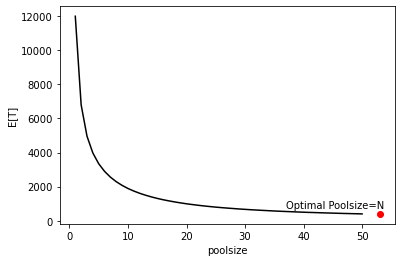
\includegraphics[width=\linewidth]{graphics/expected_cost.png}
        \caption{Optimal pool size regarding the writing transactions. $T(S_{writing})$}\label{fig:expected_cost}
    \end{subfigure}
    \qquad
    \begin{subfigure}{6cm}
        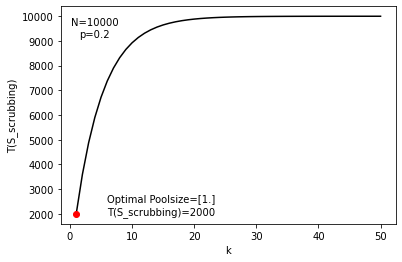
\includegraphics[width=\linewidth]{graphics/expected_scrubbing.png}
        \caption{Optimal pool size regarding the data scrubbing operations $T(S_{scrubbing})$.}\label{fig:expected_scrubbing}
    \end{subfigure}
    \qquad
    \begin{subfigure}{6cm}
        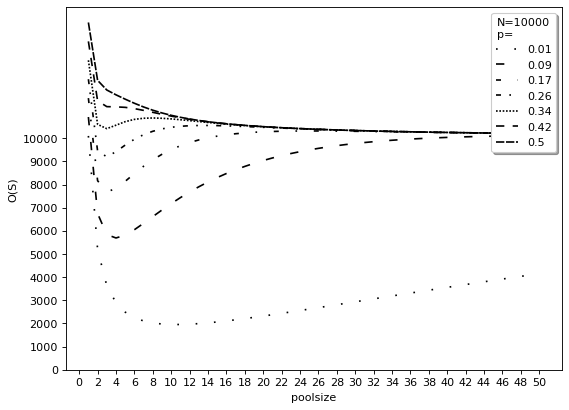
\includegraphics[width=\linewidth]{graphics/expected_operations.png}
        \caption{Optimal pool size regarding the total operations $T(S) = T(S_{writing}) + T(S_{scrubbing})$.}\label{fig:expected_operations}
    \end{subfigure}
    \caption{Comparison of optimal pool sizes \url{https://github.com/metsch/masterthesis/blob/main/src/py/rq1.ipynb}}%
    \label{fig:optimal_pool_size}%
\end{figure}
In Table \ref{tb:expected costs} and Figure \ref{fig:poolsizes} it is shown that for ingest bulks with higher prevalence of corruption smaller pool sizes are favorable.
The highest efficiency \acrshort{eff} can be achieved when the prevalence rate is the lowest, where larger pool sizes are favorable, see Figure \ref{fig:poolsizes}.
\begin{figure}[H]%
    \centering
    \caption{Optimal pool sizes $k$ with prevalence $p$ \url{https://github.com/metsch/masterthesis/blob/main/src/py/rq1.ipynb}}\label{fig:pool-sizes}
    \label{fig:poolsizes}
    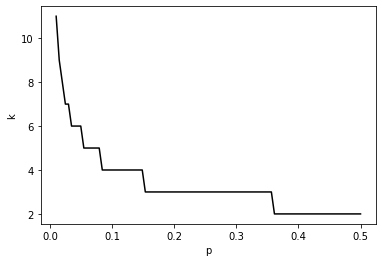
\includegraphics[width=0.5\textwidth]{graphics/poolsizes.png}
\end{figure}
\begin{table}[H]
    \caption{Efficiency \acrshort{eff} and Cost Efficiency \acrshort{cost} of two-stage-hierarchical pooling compared to individual testing \url{https://github.com/metsch/masterthesis/blob/main/src/py/rq1.ipynb}}
    \centering
    \begin{tabular}{ c c c c c}
    \label{tb:expected costs}
     N & p & k & E(\acrshort{two-stage}) & C(\acrshort{two-stage}) \\
     10000 & 0.010 & 11 & 5.16 & 11 \\ 
     \hline
     10000 & 0.05 & 5 & 2.39 & 5 \\  
     \hline
     10000 & 0.09 & 4 & 1.87 & 4 \\  
     \hline
     10000 & 0.14 & 4 & 1.62 & 4 \\  
     \hline
     10000 & 0.18 & 3 & 1.50 & 3  \\
     \hline
     10000 & 0.22 & 3 & 1.40 & 3  \\
     \hline
     10000 & 0.27 & 3 & 1.34 & 3  \\
     \hline
     10000 & 0.31 & 3 & 1.30 & 3  \\
     \hline
     10000 & 0.35 & 3 & 1.27 & 3  \\
     \hline
     10000 & 0.400 & 2 & 1.22 & 2  
    \end{tabular}
\end{table}

\textit{To what extent can pooled testing increase the efficiency and reduce cost for a fixity information storage service on the Ethereum blockchain?}

A context-sensitive approach in the medical field was proposed in 2020 were members of homogeneous groups were pooled, e.g. families, office colleagues or neighbors, and is proven to be more effective than individual testing \cite[4]{deckert2020simulation}. In this thesis, the idea of grouping similar files to increase efficiency of the pooling strategy is implemented by grouping various file extensions, estimating their prevalence in form of alterations and calculating the efficiency per file extension as presented in Equation \ref{eq:efficiency}. The dataset used is presented in Section \ref{sec:dataset}.
\begin{figure}[H]%
    \centering
    \caption{Distribution of prevalence rates $p$ \url{https://github.com/metsch/masterthesis/blob/main/src/py/rq2.ipynb}}\label{fig:p-distribution}
    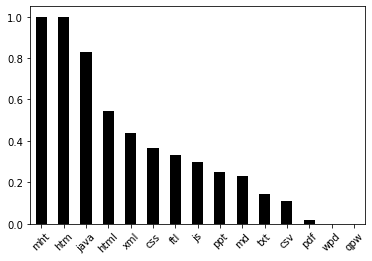
\includegraphics[width=0.5\textwidth]{graphics/p-distribution.png}
\end{figure}
In Figure \ref{fig:p-distribution}, it is shown that the volatility in the repository only affects a few file extensions, where 77 out of 90 file extension where never altered and have therefore a $p$ value of 0.00. These unaltered file extensions are grouped with a group size of $Group_N$, which results in large bulks in the ingest process that have no impact on the retrieval since I assume that no object in this particular group will be altered during the preservation process. For instance, in Table \ref{tb:efficiency}, the file extension MOV has a prevalence rate of 0.00, and therefore I can assign a group size of $N$ to reach the maximum overall efficiency.
\begin{table}[H]
    \caption{In group efficiencies of various file extensions}
    \centering
    \begin{tabular}{ c c c c c c}
    \label{tb:efficiency}
     extension & N & p & k & E(\acrshort{two-stage}) & C(\acrshort{two-stage}) \\
     \hline
     XML & 986 & 0.43 & 2 & 1.21  & 2.00 \\  
     \hline
     PDF &106 &0.01 & 8 &  3.60 & 7.57 \\
     \hline
     MD & 74 & 0.22  & 3 & 1.37 & 2.96 \\    
     \hline
     MOV&61 & 0.00 &  61 & 61.00 & 61.00 \\  
     \hline
     JAVA &47 &0.82 & 2  & 1.21 & 1.95 \\  
     \hline
     ZIP & 17 &0.00 &  17 & 17.00 & 17.00 \\
     \hline
     TXT & 14 & 0.14 &  4 & 1.33 & 3.50 \\ 
     \hline
     DOC & 13 & 0.00 &  13 & 13.00 & 13.00 \\   
     \hline
     JP2 & 12 & 0.00 &  12 & 12.00 & 12.00 \\   
     \hline
     CSS & 11 & 0.36 & 2  & 1.07 & 1.83 \\  
     \hline
     HTML & 11 & 0.54 &  2 & 1.06 & 1.83 \\   
     \hline
     JS & 10 & 0.3 & 1.08 & 2.50 
    \end{tabular}
\end{table}

To calculate the efficiency of the two stage hierarchical pooling strategy, I took the mean $p$ value of the data in Table \ref{tb:efficiency} as an estimator for the overall alteration rate which resulted in 0.06. The input for Equation \ref{eq:expected_operations} was therefore N=1560; p=0.06 and k=5.0.
With context-sensitive pooling, another increase in efficiency can be made. In Table \ref{tb:context-sensitive} I compare the two strategies presented before, with respect to Equation \ref{eq:efficiency}, where the Two-Stage-hierarchical pooling algorithm has achieved an efficiency rate of 2.24 and context-sensitive pooling has achieved an efficiency rate of 3.03. 
\begin{table}[H]
    \caption{Efficiency of context-sensitive pooling vs. two stage hierarchical pooling \url{https://github.com/metsch/masterthesis/blob/main/src/py/rq2.ipynb}}
    \centering
    \begin{tabular}{c c c}
    \label{tb:context-sensitive}
    Strategy & E(\acrshort{two-stage}) & C(\acrshort{two-stage}) \\
    Individual & 1.00 & 1.00 \\
    Two stage hierarchical &  2.81 & 4.99\\
    Context Sensitive & 3.03 & 3.25
    \end{tabular}
\end{table}

\textit{RQ 3 Given that metadata has a higher corruption rate, what effect has the split of metadata and objects on the operation cost?}
To know what effect the split off metadata has, I had to double the initial 1560 file extensions and assign the postfix .meta to the newly created rows resulting in Table \ref{tb:metadata},
\begin{table}[H]
    \caption{Arbitrary prevalence rates $p$ and $p_{meta}$ in the format-corpus dataset}
    \centering
    \begin{tabular}{c c c}
    \label{tb:metadata}
    Extension & N & p\\
    METADATA & 1560 & 0.990 \\
    XML& 986 & 0.001 \\
    PDF& 986 & 0.001 \\
    MD& 986 & 0.001 \\
    MOV& 986 & 0.001 
    \end{tabular}
\end{table}
where $p=0.005$ for each file extension and $p_{meta}=0.800$. 
I have calculated the efficiency for context-sensitive and two-stage hierarchical for various combinations of $p$ and $p_{meta}$ and the result is, that with split off metadata the context-sensitive strategy is much worse than the two-stage hierarchical algorithm.
For instance in Table \ref{tb:split-off}, the context-sensitive strategy never even reaches a 1.00 efficiency, which would state that it performs worse as the individual testing in terms of efficiency, whereas the two-stage hierarchical strategy performs better with split off metadata when the $p$ value is low enough. This is because I can assign larger group sizes when the majority of file extensions (the objects) in the dataset do have a very low prevalence rate $p$. This is due to the fact, that the average $p$ value is calculated after grouping the file extensions, where we have only one file extension where the $p$ value is very vast, the metadata.
\begin{table}[H]
    \caption{Various prevalence rates $p$ and $p_{meta}$ in the format-corpus dataset compared with the individual testing strategy \acrshort{two-stage} where 2044 operations are needed \url{https://github.com/metsch/masterthesis/blob/main/src/py/rq3.ipynb}.}
    \centering
    \begin{tabular}{c c c c c c}
    \label{tb:split-off}
    $p$ & $p_{meta}$ & E(\acrshort{cs}) & C(\acrshort{cs}) & E(\acrshort{two-stage}) & C(\acrshort{two-stage})\\
	0.001 &	0.99 &	1.76 & 3.41 &	7.17&	9.98 \\
	0.002 &	0.98 &	1.73 & 3.34 &	6.82&	9.98 \\
	0.003 &	0.98 &	1.71 & 3.29 &	6.55&	8.99 \\
	0.013 &	0.94 &	1.60 & 3.09 &	5.02&	7.99 \\
	0.014 &	0.93 &	1.60 & 3.04 &	4.93&	7.00 \\
	0.016 &	0.93 &	1.59 & 3.04 &	4.81&	7.00 \\
	0.029 &	0.87 &	1.51 & 2.91 &	3.89&	5.99 \\
	0.031 &	0.87 &	1.50 & 2.91 &	3.83&	5.99 \\
	0.032 &	0.86 &	1.50 & 2.91 &	3.77&	5.99 \\
    0.042 &	0.82 &	1.46 & 2.83 &	3.39&	4.99 \\
	0.050 &	0.80 &	1.43 & 2.83 &	3.16&	4.99
    \end{tabular}
\end{table}

\section{Dataset for context-sensitive pooling}\label{sec:dataset}
I analyzed the format-corpus\footnote{\url{https://github.com/openpreserve/format-corpus}} from Open Preserve Foundation\footnote{\url{ http://openpreservation.org/}} to get a better understanding of various file formats, mostly on how volatile they are. The latest commit for my analysis was \textit{commit 4e4b9a34540f72612ba6eab2d28bccceb7a848ae}\footnote{\url{https://github.com/openpreserve/format-corpus/commit/4e4b9a34540f72612ba6eab2d28bccceb7a848ae}} on the 16th of February. The format-corpus is well-structured in a public GitHub repo with a decent amount of reputation in form of GitHub stars, where other datasets did provide corrupt links;were not available or did expect a tedious amount of time to download and re-structure them. Convenience; diversity of file extensions; and reputation of the organization affected my decision to use the format-corpus for analysis.
For the analysis I used the python package folderstats\footnote{\url{https://pypi.org/project/folderstats/}} which transforms a directory into a pandas\footnote{\url{https://pandas.pydata.org/}} dataframe. The repository contains 1560 files with 90 distinct file extensions, e.g. 986 \textit{.xml} files which are mostly PRONOM\footnote{\url{https://www.nationalarchives.gov.uk/PRONOM/}} registry files or \textit{pom.xml} files in case of java projects. In Figure \ref{fig:extension_distribution} you can see the distribution of file extensions where \textit{.xml} files make 62.2 percent of the portion and PDF with 6.79 percent as the second-largest portion.
\begin{figure}[h]
    \caption{Distribution of file extensions in the format-corpus of Open Preserve Foundation. \url{https://github.com/openpreserve/format-corpus}}
    \label{fig:extension_distribution}
    \centering
    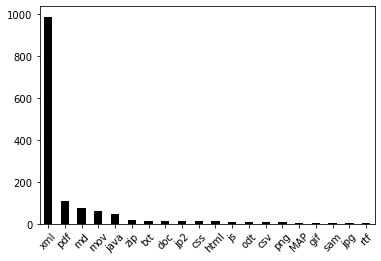
\includegraphics[width=0.5\textwidth]{extension_distribution.png}
\end{figure}

\subsection{Transformations}
To get a baseline estimate on how volatile certain extensions are due to updates and alterations, I analyzed Git logs and count how many times a file extension was involved in a commit. The resulting column \textit{positives} was always higher or equal than the occurrence of a file extension, since each file was involved in at least one commit, the initial commit of the file. To count the commits I used the python package gitphyton\footnote{\url{https://gitpython.readthedocs.io/en/stable/}} and utilized the git command --log. For each file in the repository, I fired up the command \textit{git log --oneline filename} in python which resulted in one or multiple lines of logs. Latter I used the multiline log as an input for the \textit{.splitlines()} function which results in an array of log lines, the length of this array minus 1 (the initial commit) is used to determine the new column \textit{positives} in the dataframe which shows if and how often a certain file has changed over the lifetime of the git repository. 
This method of determining the volatility of a certain file extension is by no means ideal, but there is no other method to look into how often a certain file has changed without monitoring them on a system for a certain time interval. Therefore, I have decided to use the amount of file alterations in the git repository as a rough estimate.
The prevalence rate $p$ of a file extension is calculated with $positives/N$, see Table \ref{tb:git-alterations}
\begin{table}[h]
    \caption{Volatility of certain file extensions in the format-corpus dataset}
    \centering
    \begin{tabular}{ c c c c c}
    \label{tb:git-alterations}
     extension & N & positives\\ 
     \hline
     XML & 986 & 432 & 0.43  \\
     \hline
     PDF &106 &2 &0.01  \\
     \hline
     MD & 74 & 17 & 0.22  \\   
     \hline
     MOV&61 & 0 & 0.00 \\ 
     \hline
     JAVA &47 &39&0.82 \\ 
     \hline
     ZIP & 17 &0 &0.00 \\
     \hline
     TXT & 14 & 2 & 0.14 \\
     \hline
     DOC & 13 & 0 & 0.00 \\ 
     \hline
     JP2 & 12 & 0 & 0.00 \\  
     \hline
     HTML & 11 & 6 & 0.54 \\ 
     \hline
     CSS & 11 & 4 & 0.36 \\
     \hline
     JS & 10 & 3 & 0.3 \\
    \end{tabular}
\end{table}


